\chapter{Estado del Arte}\label{chapter:state-of-the-art}

\section{Lengua de Señas}\label{section:state-of-the-art:sl}
La lengua de señas es el principal medio de comunicación para los sordos. Es una lengua que utiliza signos en lugar de sonidos para comunicarse. Los signos se producen utilizando las manos, la cara y el cuerpo. Los mismos se usan en todo el mundo y existen más de 300 variantes.
Las lenguas de señas son todas diferentes, no son inteligibles entre sí, no son universales y tienen su propia gramática y sintaxis las cuales difieren de las del lenguaje hablado.

\section{Escritura de señas Sutton}\label{section:state-of-the-art:sw}
La escritura de señas Sutton (Sutton SignWriting), comúnmente conocida como escritura de señas (SignWriting), es un sistema de escritura de lenguas de señas. Es muy específico y visualmente icónico, tanto en las formas de los personajes, que son imágenes abstractas de las manos, la cara y el cuerpo, como en su disposición espacial en la página, que no sigue un orden secuencial como las letras que forman las palabras escritas. Fue desarrollado en 1974 por Valerie Sutton, una bailarina que, dos años antes, había desarrollado la escritura danzaria (DanceWriting). Algunas formas estandarizadas más nuevas se conocen como el Alfabeto internacional de escritura por señas (ISWA por sus siglas en inglés).

\subsection{Símbolos}\label{subsection:state-of-the-art:sl:symbols}
La cantidad de símbolos es extensa y, a menudo, brinda múltiples formas de escribir un solo signo. Así como tomó muchos siglos para que la ortografía de los diversos idiomas se estandarizara, la ortografía en SignWriting aún no está estandarizada para ninguna lengua de señas.

En SignWriting, se utiliza una combinación de símbolos icónicos para formas de manos, orientación, ubicaciones corporales, expresiones faciales, contactos y movimiento[\cite{thiessen2011signwriting}][\cite{suttonsignwriting}] para representar palabras en lengua de señas.

 Sutton originalmente diseñó el guión para que se escribiera horizontalmente (de izquierda a derecha), como en su idioma nativo, y desde el punto de vista del observador, pero luego lo cambió a vertical (de arriba a abajo) y desde el punto de vista de el firmante, para ajustarse a los deseos de los escritores sordos.
 \begin{figure}[ht!]
    \centering
    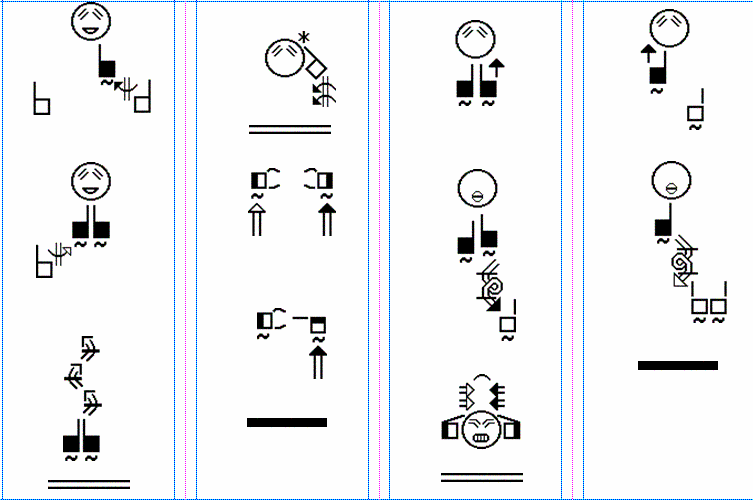
\includegraphics[width=0.6\textwidth]{Graphics/arreglo_glifos_sutton.png}
    \caption{Ejemplo de una secuencia de glifos}
    \label{fig:arreglo_glifos_sutton}
\end{figure}
 
 Dado que SignWriting representa la formación física real de los signos en lugar de su significado, no se requiere ningún análisis fonético o semántico de un idioma para escribirlo. Una persona que ha aprendido el sistema puede ''sentir'' un signo desconocido de la misma manera que una persona que habla inglés puede ''pronunciar'' una palabra desconocida escrita en el alfabeto latino, sin siquiera saber qué significa el signo.

Las palabras pueden estar escritas desde el punto de vista del firmante o del espectador. Sin embargo, casi todas las publicaciones utilizan el punto de vista del firmante y asumen que la mano derecha es dominante.

\subsection{Orientación}\label{subsection:state-of-the-art:sl:orientation}
La orientación de la palma se indica rellenando el glifo de la forma de la mano. Un glifo de contorno hueco (blanco) indica que uno está mirando hacia la palma de la mano, un glifo relleno (negro) indica que uno está mirando hacia el dorso de la mano y un sombreado dividido indica que uno está viendo la mano desde un lado. Aunque en realidad la muñeca puede girar a posiciones intermedias, en SignWriting solo se representan las cuatro orientaciones de palma, dorso y ambos lados, ya que son suficientes para representar las lenguas de señas.

Si se usa un glifo continuo, entonces la mano se coloca en el plano vertical (pared o cara) frente al firmante, como ocurre al deletrear con los dedos. Una banda borrada a través del glifo a través de los nudillos muestra que la mano se encuentra en el plano horizontal, paralela al suelo. (Si se usa uno de los glifos básicos de la forma de la mano, como el cuadrado o el círculo simple, esta banda lo divide en dos; sin embargo, si hay líneas para los dedos que se extienden desde la base, entonces se separan de la base, pero la base en sí permanece intacta). 

El diagrama de la izquierda muestra una mano BA (mano plana) en seis orientaciones. Para las tres orientaciones verticales en el lado izquierdo, la mano se sostiene frente al firmante, con los dedos apuntando hacia arriba. Los tres glifos se pueden girar, como las manecillas de un reloj, para mostrar los dedos apuntando en ángulo, hacia un lado o hacia abajo. Para las tres orientaciones horizontales en el lado derecho del diagrama, la mano se sostiene hacia afuera, con los dedos apuntando en dirección opuesta al firmante y presumiblemente hacia el espectador. También se pueden rotar para mostrar los dedos apuntando hacia un lado o hacia el firmante. Aunque se puede representar un número indefinido de orientaciones de esta manera, en la práctica solo se usan ocho para cada plano, es decir, solo se encuentran múltiplos de 45°.

\subsection{Forma de la mano}\label{subsection:state-of-the-art:sl:handshape}
Hay más de cien glifos para las formas de las manos, pero todos los que se usan en la lengua de señas americana(ASL) se basan en cinco elementos básicos:

\begin{itemize}

    \item Un cuadrado representa un puño cerrado, con los nudillos de los dedos flexionados doblados 90° para que los dedos toquen la palma y el pulgar quede sobre los dedos. Sin adornos, este cuadrado representa la mano S del deletreo manual. Modificado como se describe a continuación, indica que al menos uno de los cuatro dedos toca la palma de la mano.
    \item Un círculo representa un "puño abierto", una mano donde el pulgar y los dedos están flexionados para tocarse en sus puntas. Sin adornos, esta es la mano O del deletreo manual. Modificado, indica que al menos un dedo toca el pulgar de esta manera.
    \item Un pentágono (triángulo encima de un rectángulo), como en la ilustración utilizada para la sección de Orientación anterior, representa una mano plana, donde todos los dedos están rectos y en contacto. Esto es similar a la mano B del deletreo manual, aunque sin que el pulgar cruce la palma.
    \item Una forma de 'C' representa una mano donde el pulgar y los dedos están curvados, pero no lo suficiente como para tocarlos. Esto se usa para la mano C del deletreo manual y se puede modificar para mostrar que los dedos están separados.
    \item Una forma en ángulo, como una L gorda, muestra que los cuatro dedos son planos (derechos y en contacto), pero doblados a 90° del plano de la palma. No aparece como una forma simple, sino que debe incluir una indicación de dónde está el pulgar, ya sea hacia un lado o tocando las puntas de los dedos.

\end{itemize}

\begin{figure}[ht!]
    \centering
    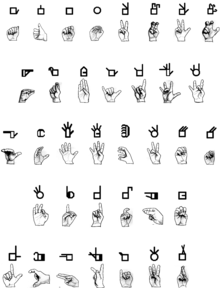
\includegraphics[width=0.6\textwidth]{Graphics/suttonhandshape.png}
    \caption{Formas de las manos y su representación en SignWriting}
    \label{fig:handshape}
\end{figure}

Una línea a la mitad del cuadrado o pentágono muestra el pulgar en la palma de la mano. Estas son la E, B y (con los dedos separados) 4 manos de deletreo manual.

Estas formas básicas se modifican con líneas que sobresalen de sus caras y esquinas para representar dedos que no están colocados como se describe arriba. Las líneas rectas representan dedos rectos (estos pueden estar en ángulo para indicar que no están alineados con la palma; si apuntan hacia o lejos del firmante, tienen forma de diamante en la punta); líneas curvas para dedos curvos (en forma de copa); líneas ganchudas para dedos ganchudos; líneas de ángulo recto, para dedos doblados en una sola articulación; y líneas cruzadas, para dedos cruzados, como se muestra en el gráfico de la derecha. El pentágono y C solo se modifican para mostrar que los dedos están separados en lugar de estar en contacto; el ángulo solo se modifica para mostrar si el pulgar toca las puntas de los dedos o sobresale hacia un lado. Aunque se pueden hacer algunas generalizaciones para las docenas de otros glifos, que se basan en el círculo y el cuadrado, los detalles son algo idiosincrásicos y cada uno debe memorizarse.

\subsection{Movimiento de los dedos}\label{subsection:state-of-the-art:sl:finger_movement}
Solo hay unos pocos símbolos para el movimiento de los dedos. Pueden duplicarse para mostrar que el movimiento se repite.

Una bala sólida representa flexionar la articulación media de un dedo o dedos, y una bala hueca representa enderezar un dedo flexionado. Es decir, una mano 'D' con una bala sólida significa que se convierte en una mano 'X', mientras que una mano 'X' con una bala hueca significa que se convierte en una mano 'D'. Si los dedos ya están flexionados, entonces una bala sólida muestra que aprietan. Por ejemplo, un cuadrado (puño cerrado, mano 'S') con viñetas sólidas dobles es el signo de 'leche' (icónicamente apretando una ubre).

\begin{figure}[ht!]
    \centering
    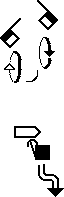
\includegraphics[scale=0.5]{Graphics/finger_movement.png}
    \caption{Ejemplo de movimiento de los dedos en SignWriting}
    \label{fig:finger_movement}
\end{figure}

Un cheurón que apunta hacia abajo representa la flexión de los nudillos, mientras que un cheurón que apunta hacia arriba ( $\wedge$ ) muestra que los nudillos se enderezan. Es decir, una mano 'U' con un cheurón hacia abajo se convierte en una mano 'N', mientras que una mano 'N' con un cheurón hacia arriba se convierte en una mano 'U'.

Un zigzag como dos cheurones ($ \wedge\wedge $) unidos significa que los dedos se flexionan repetidamente y sincronizados. Un zigzag de doble línea significa que los dedos se retuercen o aletean sin sincronización.

\subsection{Movimiento de las manos}\label{subsection:state-of-the-art:sl:hand_movement}
Cientos de flechas de varios tipos se utilizan para indicar el movimiento de las manos a través del espacio. La notación de movimiento se vuelve bastante compleja, y debido a que es más exacta de lo que necesita ser para cualquier lengua de señas, diferentes personas pueden optar por escribir el mismo signo de diferentes maneras.

Para el movimiento con la mano izquierda, la punta de flecha en forma de $ \bigtriangleup $ es hueca (blanca); para el movimiento con la mano derecha, es sólido (negro). Cuando ambas manos se mueven como una sola, se usa una punta de flecha abierta (en forma de $ \wedge $ ).

Al igual que con la orientación, las flechas de movimiento distinguen dos planos: el movimiento en el plano vertical (arriba y abajo) está representado por flechas con dos ejes, como en la parte inferior del diagrama de la izquierda, mientras que las flechas de un solo eje representan el movimiento paralelo al suelo ( de ida y vuelta). Además, el movimiento en un plano diagonal utiliza flechas de doble tallo modificadas: una barra transversal en el tallo indica que el movimiento es hacia arriba o hacia abajo, y un punto sólido indica un movimiento de aproximación. El movimiento de ida y vuelta que también pasa por encima o por debajo de algo utiliza flechas modificadas de un solo tallo, con la parte de la flecha que representa el movimiento cercano más gruesa que el resto. Estos son icónicos, pero convencionalizados, por lo que deben aprenderse individualmente.

Los movimientos rectos son en una de las ocho direcciones para cualquier plano, como en las ocho direcciones principales de una brújula. Una flecha recta larga indica movimiento desde el codo, una flecha corta con una barra transversal detrás indica movimiento desde la muñeca y una flecha corta simple indica un movimiento pequeño. (Duplicados, en direcciones opuestas, estos pueden mostrar movimientos de cabeza desde la muñeca). Una flecha curva secundaria que cruza la flecha principal muestra que el brazo gira mientras se mueve. (Duplicadas, en direcciones opuestas, pueden mostrar el temblor de la mano). Las flechas pueden girar, curvarse, zigzaguear y hacer bucles.

\subsection{Movimiento de la cabeza y los ojos}\label{subsection:state-of-the-art:sl:head_eye_shoulders}
Las flechas en la cara a la altura de los ojos muestran la dirección de la mirada. 

\subsection{Símbolos de Contacto}\label{subsection:state-of-the-art:sl:contact_symbol}

Seis glifos de contacto muestran el contacto de la mano con la ubicación de la señal. Es decir, un glifo de forma de mano ubicado al costado de la cara, junto con un glifo de contacto, indica que la mano toca el costado de la cara. La elección del glifo de contacto indica la forma del contacto:
\begin{itemize}
	\item un asterisco ($ \ast $ o $ * $) por simplemente tocar el lugar;
    \item un signo más ($ + $) para agarrar el lugar (generalmente la otra mano);
    \item un signo de hashtag o almohadilla ($ \sharp $) para marcar el lugar;
    \item un círculo con un punto dentro ($ \odot $) para cepillar el lugar y luego dejarlo;
    \item una espiral (o puede aproximarse con $ @ $) para frotar el lugar y no salir; si no hay flecha adicional, se entiende que está en círculos; y
    \item dos barras a cada lado de un símbolo de contacto ($ |\ast| $) para indicar que el contacto ocurre entre elementos del lugar de contacto; generalmente entre los dedos, o dentro de una forma de mano circular. (Un contacto que no sea el asterisco básico rara vez se usa entre barras).
\end{itemize}

\begin{figure}[ht!]
    \centering
    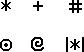
\includegraphics[width=0.6\textwidth]{Graphics/contact_symbols.png}
    \caption{Ejemplo de símbolos de contacto}
    \label{fig:contact_symbols}
\end{figure}

\subsection{Ubicación}\label{subsection:state-of-the-art:sl:location}

Si la mano que firma se encuentra en la otra mano, el símbolo de la misma es una de las formas de mano anteriores. En la práctica, solo ocurre un subconjunto de las formas de manos más simples.

Se utilizan símbolos adicionales para representar ubicaciones de signos en la cara o partes del cuerpo distintas de las manos. Un círculo muestra la cabeza.

\subsection{Expresión}\label{subsection:state-of-the-art:sl:expression}
Hay símbolos para representar los movimientos faciales que se usan en varias lenguas de señas, incluidos los ojos, las cejas, los movimientos de la nariz, las mejillas, los movimientos de la boca y los cambios en la respiración. También se puede mostrar la dirección del movimiento de la cabeza y la mirada.

\subsection{Movimiento corporal}\label{subsection:state-of-the-art:sl:body_movement}
Los hombros se muestran con una línea horizontal. Se pueden agregar flechas pequeñas para mostrar el movimiento del hombro y el torso. Se pueden agregar brazos e incluso piernas si es necesario.

\subsection{Prosodia}\label{subsection:state-of-the-art:sl:prosody}

También hay símbolos que indican la velocidad del movimiento, si el movimiento es simultáneo o alterno, y la puntuación.

\subsection{Puntuación}\label{subsection:state-of-the-art:sl:punctuation}
Existen varios símbolos de puntuación que corresponden a comas, puntos, signos de interrogación y exclamación y otros símbolos de puntuación de otras escrituras. Estos se escriben entre signos, y las líneas no se rompen entre un signo y su siguiente símbolo de puntuación.




\section{Tecnología de avatares}\label{section:state-of-the-art:avatars}


La traducción automática de lenguas de señas, aplicando la tecnología de generación de avatares, ha sido empleada en proyectos como ViSiCAST  y eSIGN, apoyados por la Unión Europea [\cite{visicast_at_uea_2021}] [\cite{esign_at_uea_2021}]. 

Se utilizan para traducir de las lenguas habladas a las lenguas de señas, lo cual solamente concierne la parte de el avatar en sí.

Las animaciones para las señas individuales son generadas basándose
en las señas no manuales de datos complementarios y en señas individuales. 

Los procesos para generar los avatares incluyen una serie de pasos bastante complejos.
 
Los aspectos referentes a la velocidad, el ritmo y el tamaño deben ser tomados en
consideración utilizando reglas para controlarlos, ser configurados por un humano o
como resultado de un modelo de aprendizaje de máquina [\cite{nguyen2021automatic}].

Otro de los usos que tienen estos métodos es lograr el anonimato en los videos y cabe remarcar que  son nuevos comparándolos relativamente con otros métodos de traducción automática de lenguas de señas [\cite{kang2010effect}] [\cite{saragih2011real}].

Uno de los más grandes desafíos es que los avatares luzcan como humanos. En diversos estudios se comparan los gestos de los avatares con los gestos de los
humanos incluyendo algunos trabajos que han obtenido buenos resultados en Reino Unido en cuanto a generar dichos avatares con rasgos humanos[\cite{stoll2018sign}] y  en Corea, usando el mismo corpus del trabajo anterior, se han logrado avances en un enfoque no autorregresivo para lograr resultados incluso mejores[\cite{hwang2021non}].

 Entre las tecnologías más utilizadas para la generación de avatares por animación se encuentran:
 \begin{itemize}
 \item  Unity
 \item Unreal 4
 \item Blender
 \item Maya3D 
 \item DirectX
 \end{itemize}  
 
 Se han desarrollado lenguajes de marcado para automatizar la generación de avatares de una forma dinámica y flexible [\cite{latoschik2017effect}] [\cite{aneja2019high}].

El estado del arte en la generación de avatares no está completamente automatizado, la mayoría de las partes del proceso de generación incluyen intervención humana para lograr buenos resultados.

Gran parte de las investigaciones miden la calidad de las animaciones de avatares de forma perceptual y de estudios comprensivos con participantes sordos-mudos, incluyendo investigaciones metodológicas y recursos compartidos [\cite{huenerfauth2006generating}] [\cite{kacorri2017regression}].


\section{Producción de Lengua de Señas}\label{section:state-of-the-art:slp}
La producción de lengua de señas(o SLP por sus siglas en inglés) ha tenido una adecuada trayectoria en cuanto a proyectos basados en avatares se refiere, los cuales generan señas parecidas a las realizadas por los humanos, pero se basan en búsqueda de frases y diccionarios de movimientos predefinidos [\cite{McDonald2015AnAT}], o requieren captura de movimiento costosa o frases pregrabadas [\cite{Lu2011DataDrivenSO}]. Con los avances recientes en el aprendizaje profundo, Stoll et al. Alabama. [\cite{stoll2018sign}] proponen el primer modelo SLP para traducir texto en glosario de palabras y mapearlas a las poses de signos correspondientes. Zelinka y Kanis [\cite{Zelinka_2020_WACV}] proponen el primer modelo SLP de extremo a extremo de longitud fija y  también proponen un método de descenso de gradiente para el refinamiento de los esqueletos generados. Recientemente, [\cite{Jiang2021SkeletorST}] proponen un transformador(transformer en inglés), basado en estos modelos de Zelinka, el cual refina el esqueleto levantado en 3D con un enfoque de entrenamiento parecido a BERT . [\cite{saunders2020progressive}] proponen Transformador Progresivo (PT), que utiliza un esquema de contracodificación para aprender directamente el mapeo entre lenguaje hablado y secuencia de poses de señas.

\subsection{Redes Neuronales Convolucionales}\label{subsection:state-of-the-art:slp:CNN}
Uno de los bloques básicos de los métodos utilizados en el razonamiento visual son las capas convolucionales. Usando estas capas, las redes neuronales convolucionales(CNN por sus siglas en íngles) modelan de manera efectiva la estructura de las imágenes[\cite{LeCun1998GradientbasedLA}]. En cuanto a la producción de lengua de señas, las convolucionales son la mismísima base de los modelos propuestos. Sin embargo, el desarrollo de las CNN enfrenta inconvenientes con respecto al campo receptivo limitado, introducido como el tamaño del núcleo. Como solución, ideas como usar muchas más capas convolucionales, aumentar el tamaño del núcleo, entre otras. Otro inconveniente importante de las CNNs es la falta de aprendizaje temporal correspondiente a secuencias de imágenes. Lo cual es propiamente resuelto utilizando a las convolucionales de tres dimensiones(3DCNN por sus siglas) como alternativa ante el modelado de tipo recurrente. Variedad de modelos han sido propuestos para problemas relacionados con la lengua de señas en los cuales se utilizan las 3DCNN [\cite{Sharma2021ASL3DCNNAS}] [\cite{AlHammadi2020HandGR}] [\cite{2019ProceedingsOT}]. Sin embargo esta última variante de las convolucionales no es generalmente tan poderosa como los modelos específicos para aprendizaje secuencial como las Redes Neuronales Recurrentes, Gran Memoria de Corto Plazo y las Unidades con Escotilla Recurrentes(GRU).

\subsection{Redes Recurrentes}\label{subsection:state-of-the-art:slp:LSTM}
La primera intuición acerca de los modelos recurrentes es que modelan la representación temporal de datos secuenciales tales como vídeos(secuencia de imágenes). Las redes neuronales recurrentes profundas han demostrado ser exitosas en diversas tareas de aprendizaje de secuencias, como lo son en la traducción automática (anteriormente tratada en el capítulo), reconocimiento del habla, subtitulado de vídeo, predicción de vídeo, reconocimiento de lengua de señas [\cite{leynier-lsc-2021}] y, como no, en la tarea que nos deviene que es el SLP. Sin embargo, existen limitaciones para estas redes, como es el caso del gradiente explosivo y desvaneciente. Para evitar este tipo de fallas, las redes neuronales recurrentes fueron extendidas a unos modelos más sofisticados como lo son las LSTM y las GRU. Diferentes trabajos han explorado modificaciones de los anteriores modelos extendidos, tales como:
\begin{itemize}

\item aplicar los modelos basados en LSTM al espacio de las imágenes[\cite{Shi2015ConvolutionalLN}]
\item usando LSTM multidimensionales(MD-LSTM)[\cite{Graves2007MultidimensionalRN}]
\item  apilando capas de LSTM para incluir correlaciones espacio-temporales abstractas[\cite{Finn2016UnsupervisedLF}]
\end{itemize} 

Aunque últimamente los modelos transformadores han obtenido muy buenos resultados en el ultimo lustro dado su mecanismo de auto-atención y cómputo paralelo. Cabe destacar que en la mayoría de los modelos para SLP se emplea un modelo recurrente por la necesidad de una representacion temporal de la secuencia de datos



\section{Reconocimiento de la Lengua de Señas}\label{section:state-of-the-art:slr}
El reconocimiento de la lengua de señas es ampliamente usado. Se emplea en la identificación de gestos de las lenguas de señas usando conjuntos de datos existentes
previamente. Las dos manos, la cabeza, los ojos, los
labios y el cuerpo  son, en esencia, lo utilizado en las lenguas de señas para realizar infinidad de gestos dedicados a funciones lingüísticas [\cite{sandler2012dedicated}]. Al ser los gestos una parte fundamental de este tipo de lenguas, se requiere de su reconocimiento específico de ellos. Los métodos de reconocimiento de gestos se pueden dividir en dos grandes grupos, en dependencia si utilizan un enfoque basado en hardware como Kinect u otros tipos de sensores, o un enfoque basado en software [\cite{mitra2007gesture}].

Dentro de este segundo enfoque destaca la detección de gestos por MediaPipe Holistic de Google logrando muy buenos resultados en dichas tareas [\cite{mediapipe_2020}] [Fig \ref{fig:mediapipe} ].


\begin{figure}[ht!]
    \centering
    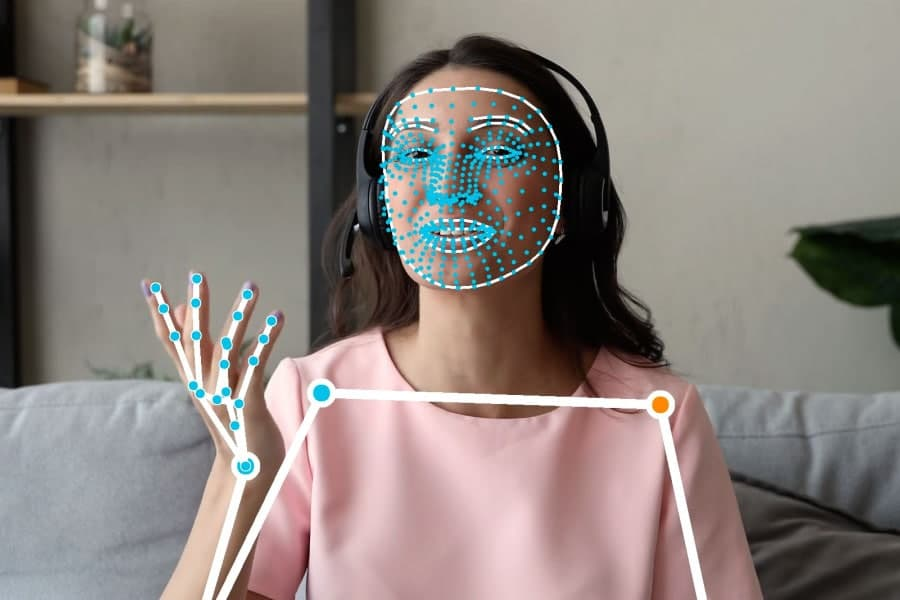
\includegraphics[width=0.6\textwidth]{Graphics/mediapipe.png}
    \caption{Software MediaPipe Holistic de Google}
    \label{fig:mediapipe}
\end{figure}


\section{Investigaciones y proyectos relacionados con la Lengua de Señas Cubana}\label{section:state-of-the-art:cubana}
En el área de las tecnologías de la información y las
comunicaciones sobre la Lengua de Señas Cubana  el autor refiere otros 2 proyectos y/o trabajos.
 
 El desarrollo de una aplicación móvil [Fig. \ref{fig:app_cubana}] para dispositivos con sistema operativo Android. Una aplicación multimedia enfocada en las familias con niños sordo-mudos, para brindarles el vocabulario necesario para interactuar con sus hijos [\cite{android_app_lsc}] y la tesis de grado referente al reconocimiento de la lengua de señas cubana usando métodos de traducción basados en inteligencia artificial y aprendizaje de maquina [\cite{leynier-lsc-2021}]

\begin{figure}[ht!]
    \centering
    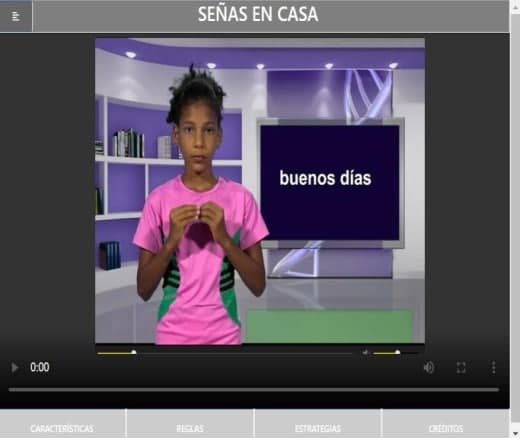
\includegraphics[width=0.6\textwidth]{Graphics/app_cubana.png}
    \caption{ Aplicación Android para la LSC [\cite{android_app_lsc}]}
    \label{fig:app_cubana}
\end{figure}

Se constata la existencia de una única investigación previa relacionada con la interpretación automática de la Lengua de Señas Cubana [\cite{leynier-lsc-2021}] pero ninguna en su contraparte de SLP.